% ****************************************************************************************************
\chapter{Problembeschreibung} \label{ch:problem}
Das folgende Kapitel beschäftigt sich mit dem \IT{Business Understanding}.
Zuerst wird in \autoref{ch4:aufbau} der Ablauf und Aufbau am Windrad gezeigt und in \autoref{ch4:requirements} werden die Anforderungen abgeleitet.
Zuletzt werden in \autoref{ch4:questions} die daraus resultierenden Fragen aufgestellt, die diese Arbeit beantworten soll.

% ****************************************************************************************************
\section{Aufbau und Ablauf am Windrad}
\label{ch4:aufbau}

\begin{figure}[ht]
    \begin{small}
        \begin{center}
            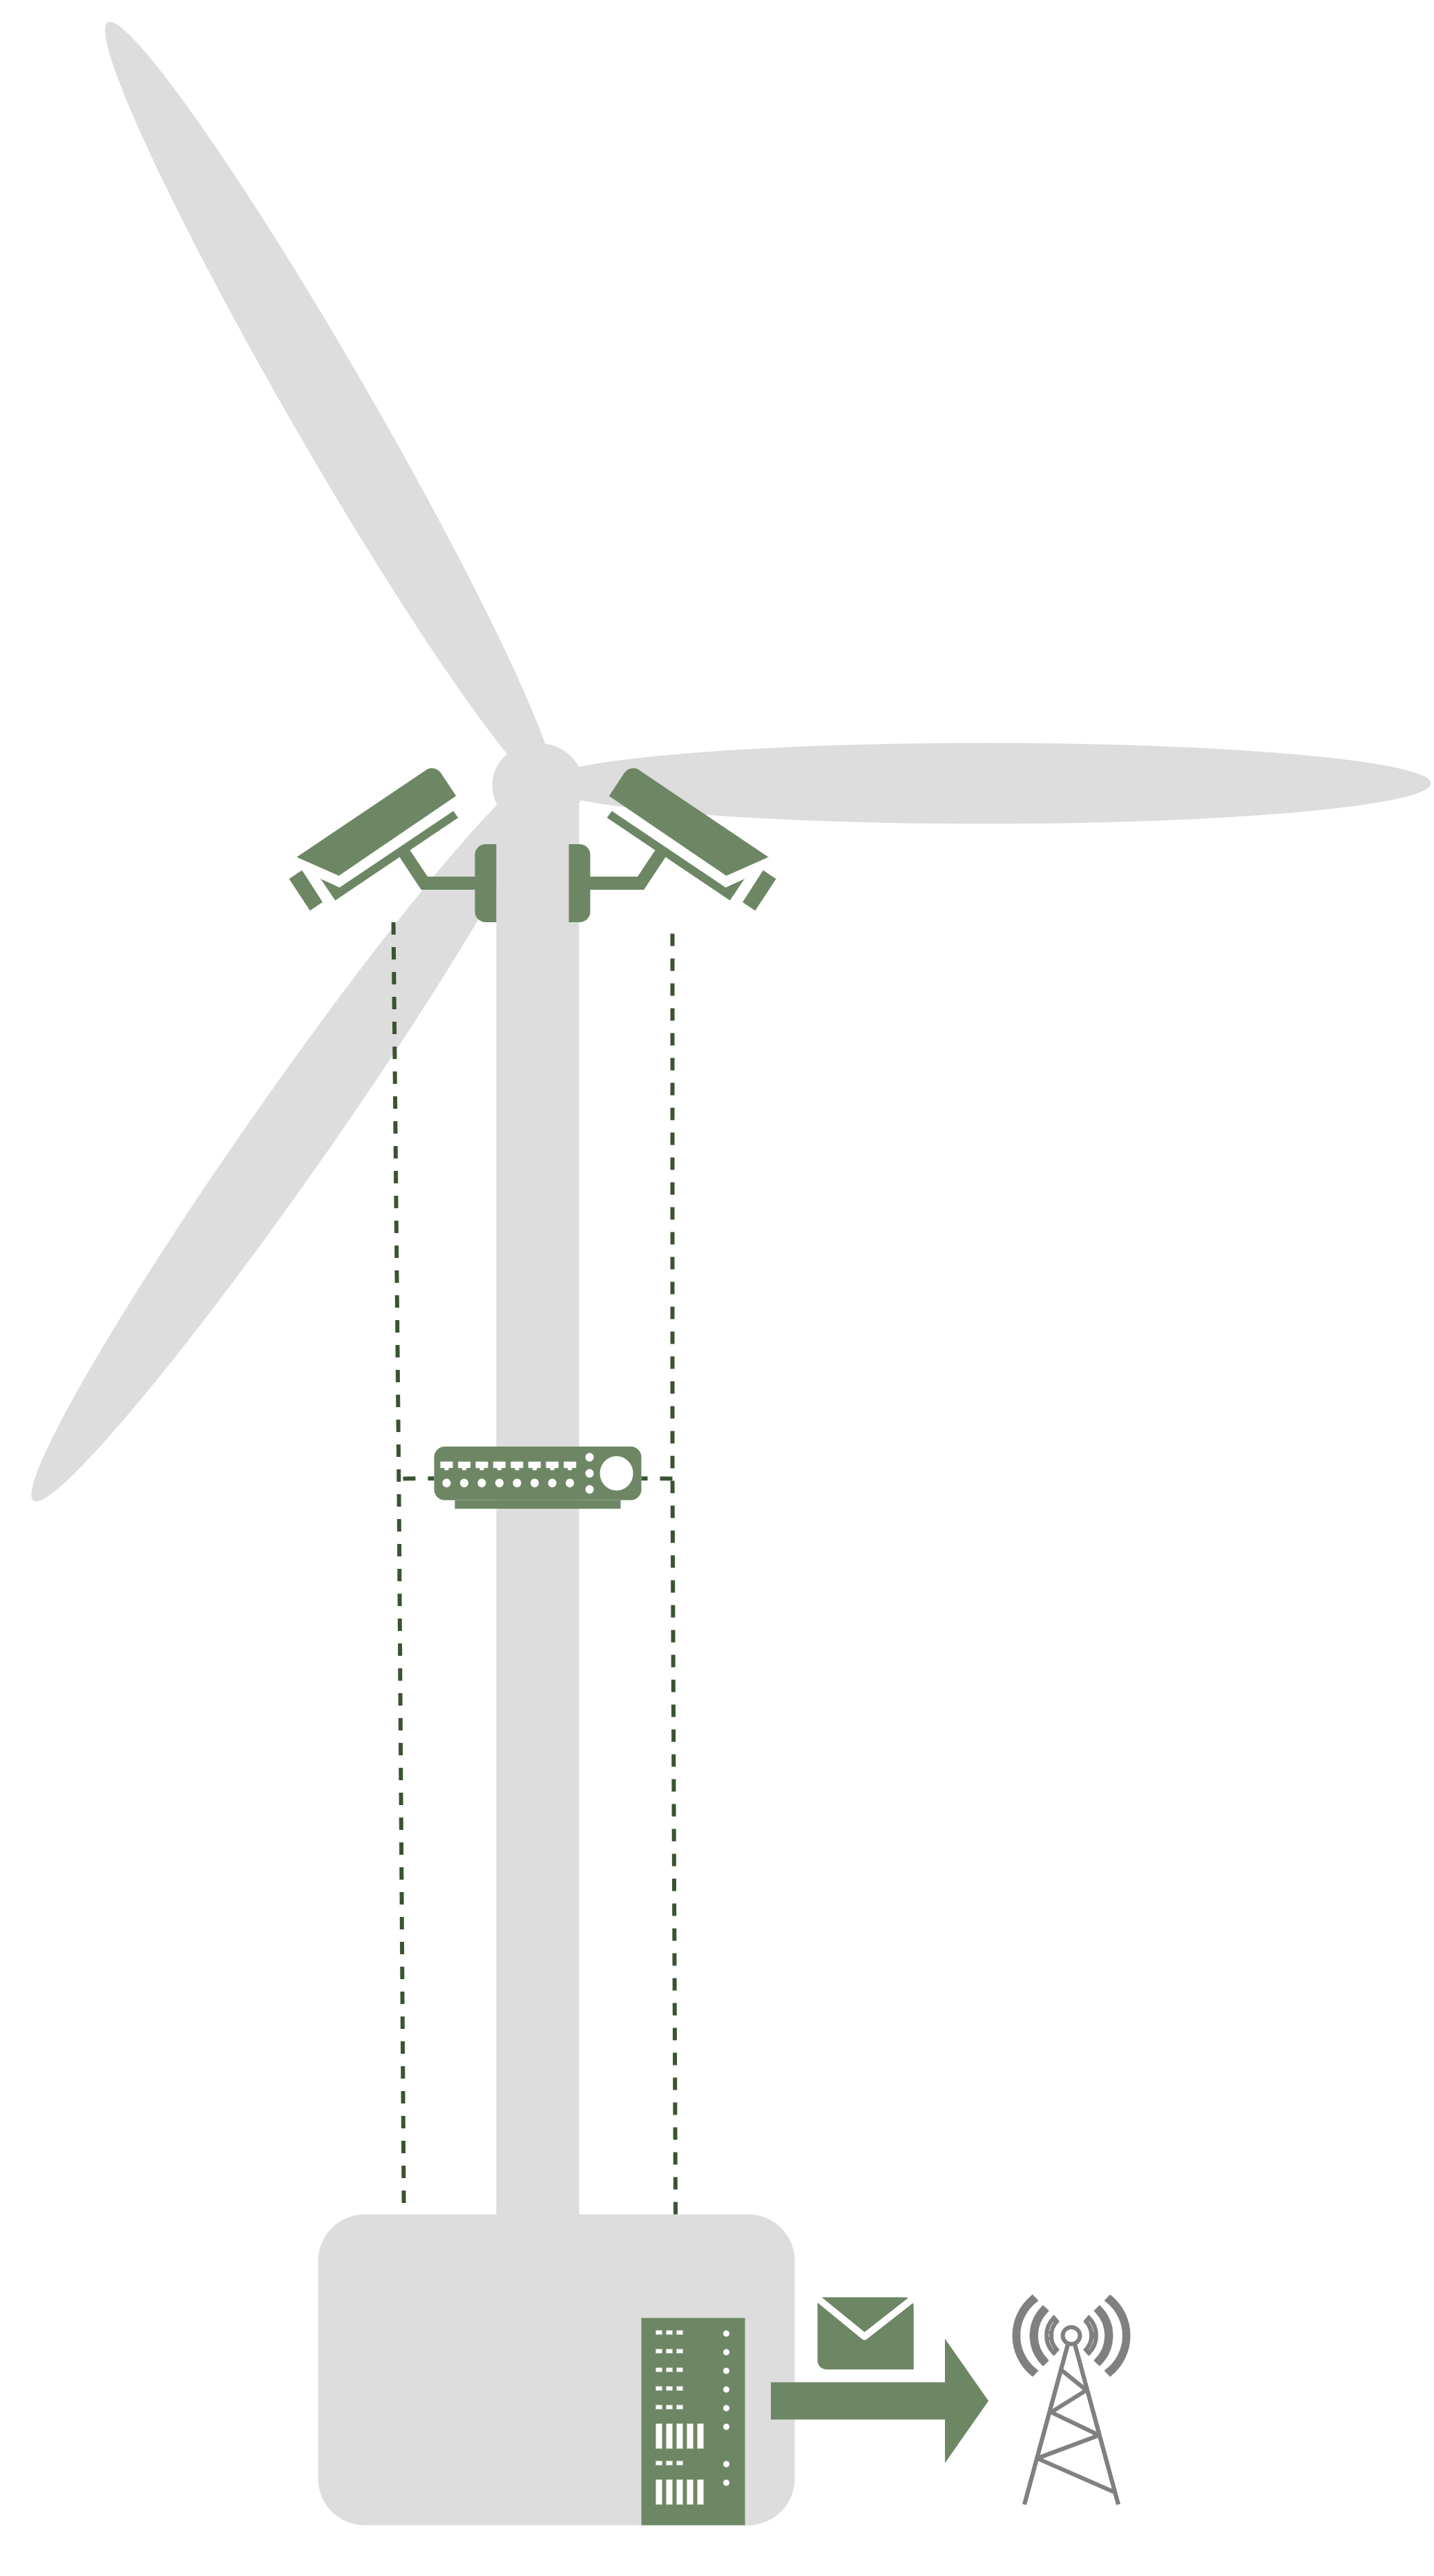
\includegraphics[height=0.5\textheight]{figures/architecture/windrad.png}
        \end{center}
        \caption{Aufbau am Windrad}
        \label{ch4:fig:windrad}
    \end{small}
\end{figure}

\autoref{ch4:fig:windrad} zeigt den Aufbau am Windrad.
Mehrere Kameras - für eine \ang{360} Überwachung - sind an dem Windrad befestigt und mit einem Computer verbunden.
Dieser steht in einer Kabine, die ihn vor Umwelteinflüssen wie Regen schützt.
Er führt die Analyse der Bilder aus und gibt entsprechend per E-Mail an den Windparkbetreiber einen Alarm über Mobilfunk ab.
Eine weitere Person entscheidet daraufhin über eine vorübergehende Abschaltung der \ac{WEA}.
Aus Zeitgründen werden für die Alarmgabe in dieser Arbeit nur zwei Konzepte angerissen.

Für die Verbindung zwischen Kamera und Computer würde sich \textit{Power over Ethernet} anbieten, da es
\begin{enumerate}[i)]
    \item Strom \& hohe Datenraten in einem Kabel überträgt und
    \item eine Reichweite von \SI{100}{\metre} ermöglicht.
\end{enumerate}
Für eine verlustfreie Erweiterung der Reichweite kann ein \textit{Repeater} als \textit{Bridge} eingefügt werden.

\bigskip
Um eine Bodenbewirtschaftungsmaßnahme bzw. einen Traktor zu erkennen, ist seine Größe auf dem Bild wichtig.
Dabei entscheidet nicht nur die Auflösung der Kamera darüber, auf wie viele Pixel er abgebildet wird.

Je nach Höhe der Kamera verkürzt sich die Distanz zum Objekt und es erscheint größer.
Ist hingegen der Öffnungswinkel größer, wird ein größerer Bereich aufgenommen und das Objekt nimmt einen kleineren Teil im Bild ein.

Bei der Wahl der Kamera besteht also eine starke Kopplung zwischen
\begin{enumerate*}[i)]
    \item{Montagehöhe der Kameras},
    \item{Öffnungswinkel der Kameras und}
    \item{Auflösung der Kameras}
\end{enumerate*}.
Je nach Wahl der ersten zwei Parameter kann ein unbewachter Bereich entstehen (gekennzeichnet als rotes Dreieck in \autoref{ch4:fig:dead}).
Dies ist jedoch kein Problem, da die Objekte zuerst den überwachten Bereich durchqueren müssen und dabei gesichtet werden.
Problematisch wird es, wenn im Sichtfeld Wälder stehen, weshalb die Kamera möglichst hoch aufgehangen werden sollte.

\begin{figure}[ht]
    \begin{small}
        \begin{center}
            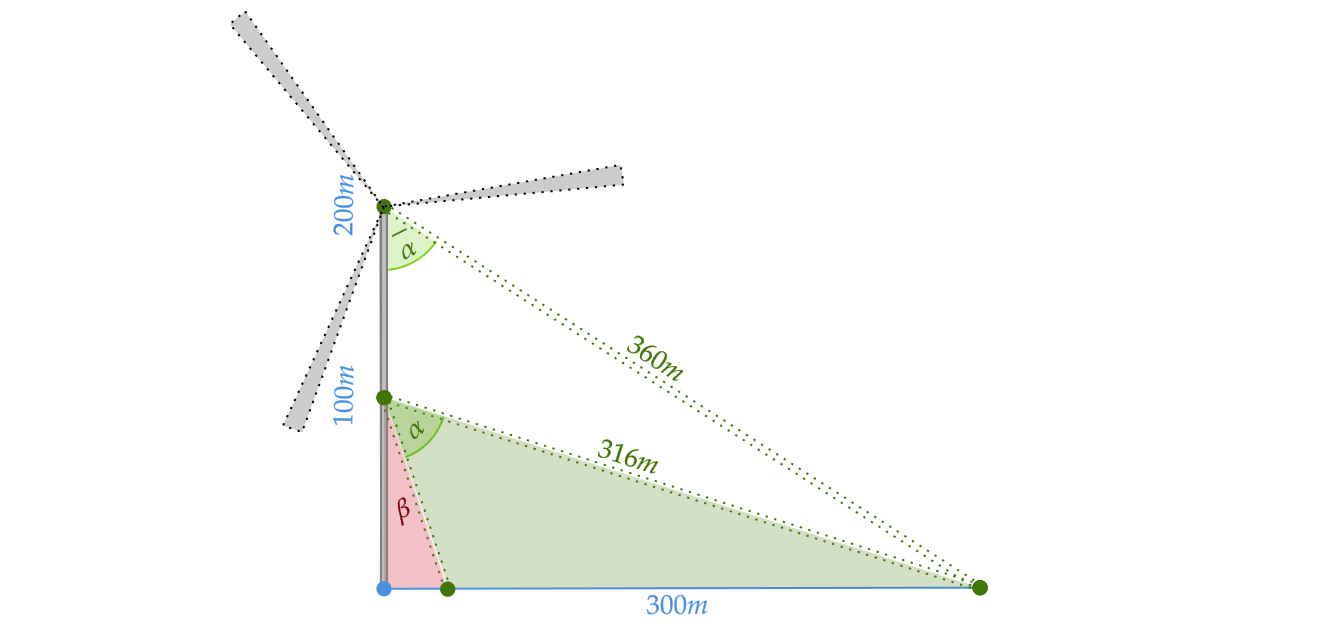
\includegraphics[width=0.95\textwidth]{figures/camera/vertical.png}
        \end{center}
        \caption[Toter Winkel bei verschiedenen Montagehöhen]{Toter Winkel von $\beta = \SI{21}{\degree}$ bei einer Montagehöhe von \SI{100}{\metre} und einem Öffnungswinkel von $\alpha = \SI{50}{\degree}$.
        Der Winkel zwischen Windrad und \SI{300}{\metre} Grenze ergibt sich aus $\arctan\left(\frac{300}{height}\right)$.}
        \label{ch4:fig:dead}
    \end{small}
\end{figure}

\section{Anforderungen} \label{ch4:requirements}
Im Folgenden werden die funktionalen Anforderungen an das System dargelegt:
\begin{itemize}
    \item In einem Radius von $300$ Metern um das Windrad, müssen Traktoren erkannt werden.
    \item Die Traktoren müssen zu verschiedenen Wetterbedingungen erkannt werden.
        Insbesondere sollen hier die Wettereinwirkungen Regen und Nebel getestet werden.
    \item Die Traktoren müssen zu verschiedenen Tageszeiten erkannt werden.
    \item Ein Alarm muss nach spätestens einem fünf minütigen Aufenthalts des Traktors abgegeben werden.
\end{itemize}

Weiter gelten folgende nicht-funktionale Anforderungen:
\begin{itemize}
    \item Die einzelnen Komponenten müssen für diese Arbeit in der Programmiersprache Python entwickelt werden, da diese im Bereich Data Science weit verbreitet ist und ein schnelles Prototyping ermöglicht.
    \item Die einzelnen Komponenten sollen einfach ausgetauscht werden können.
    \item Das Konzept soll möglichst energiesparend sein, um Kosteneffizient für den Betreiber zu sein.
\end{itemize}


\section{Forschungsfrage} \label{ch4:questions}
Diese Arbeit soll folgende Fragen beantworten:
\begin{itemize}
    \item Können mit dem kommendem Konzept Traktoren zuverlässig erkannt werden?
\end{itemize}

Werden die Traktoren erkannt, sollen diese Folgefragen beantwortet werden:
\begin{itemize}
    \item Wie schnell können Traktoren sinnvoll erkannt werden?
    \item Wie groß muss der Traktor auf dem Bild sein, um~
    \begin{enumerate*}[i)]
        \item gefunden zu werden und
        \item richtig klassifiziert zu werden?
    \end{enumerate*}
\end{itemize}

Die Antwort auf die nötige Mindestgröße der Traktoren im Bild hat Einfluss auf die Wahl der Kamera (siehe \autoref{apx:res}).

% \begin{mdframed}
%     \textbf{Exkurs: Wahl der Kamera} \\
%     \begin{itemize}
%         \item Wetterfest (\textsc{IP67} Zertifikat)
%         \item Öffnungswinkel:
%             Bei zu kleinem vertikalem Öffnungswinkel $\alpha$ kann ein totes Sichtfeld wie in \autoref{ch4:fig:dead} entstehen: \\
%             $\beta = \arctan\left({\frac{breite}{h"ohe}}\right) - \alpha$

%             \begin{center}
%                 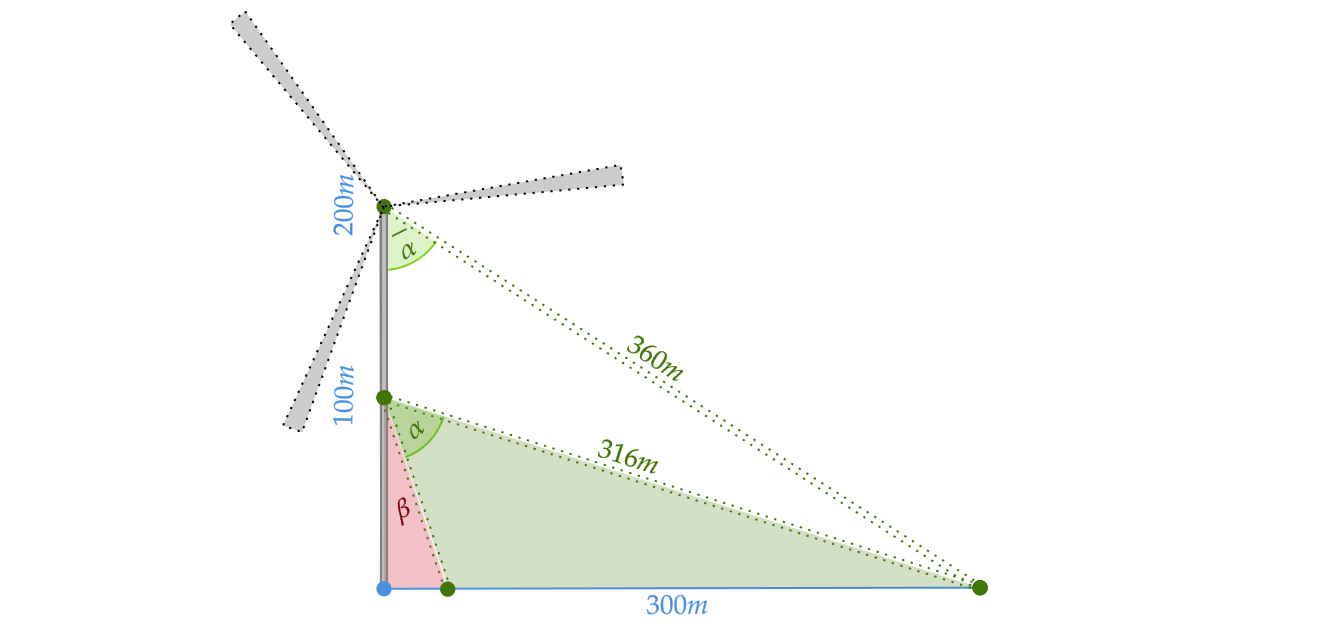
\includegraphics[width=0.9\textwidth]{figures/camera/vertical.png}
%                 \captionof{figure}{Toter Winkel}
%                 \label{ch4:fig:dead}
%             \end{center}
%         \item Auflösung:
%             $B = 2* tan(\alpha/2)*A$,
%             $aufl"osung = 32px*\frac{B}{5m}$

%             \begin{center}
%                 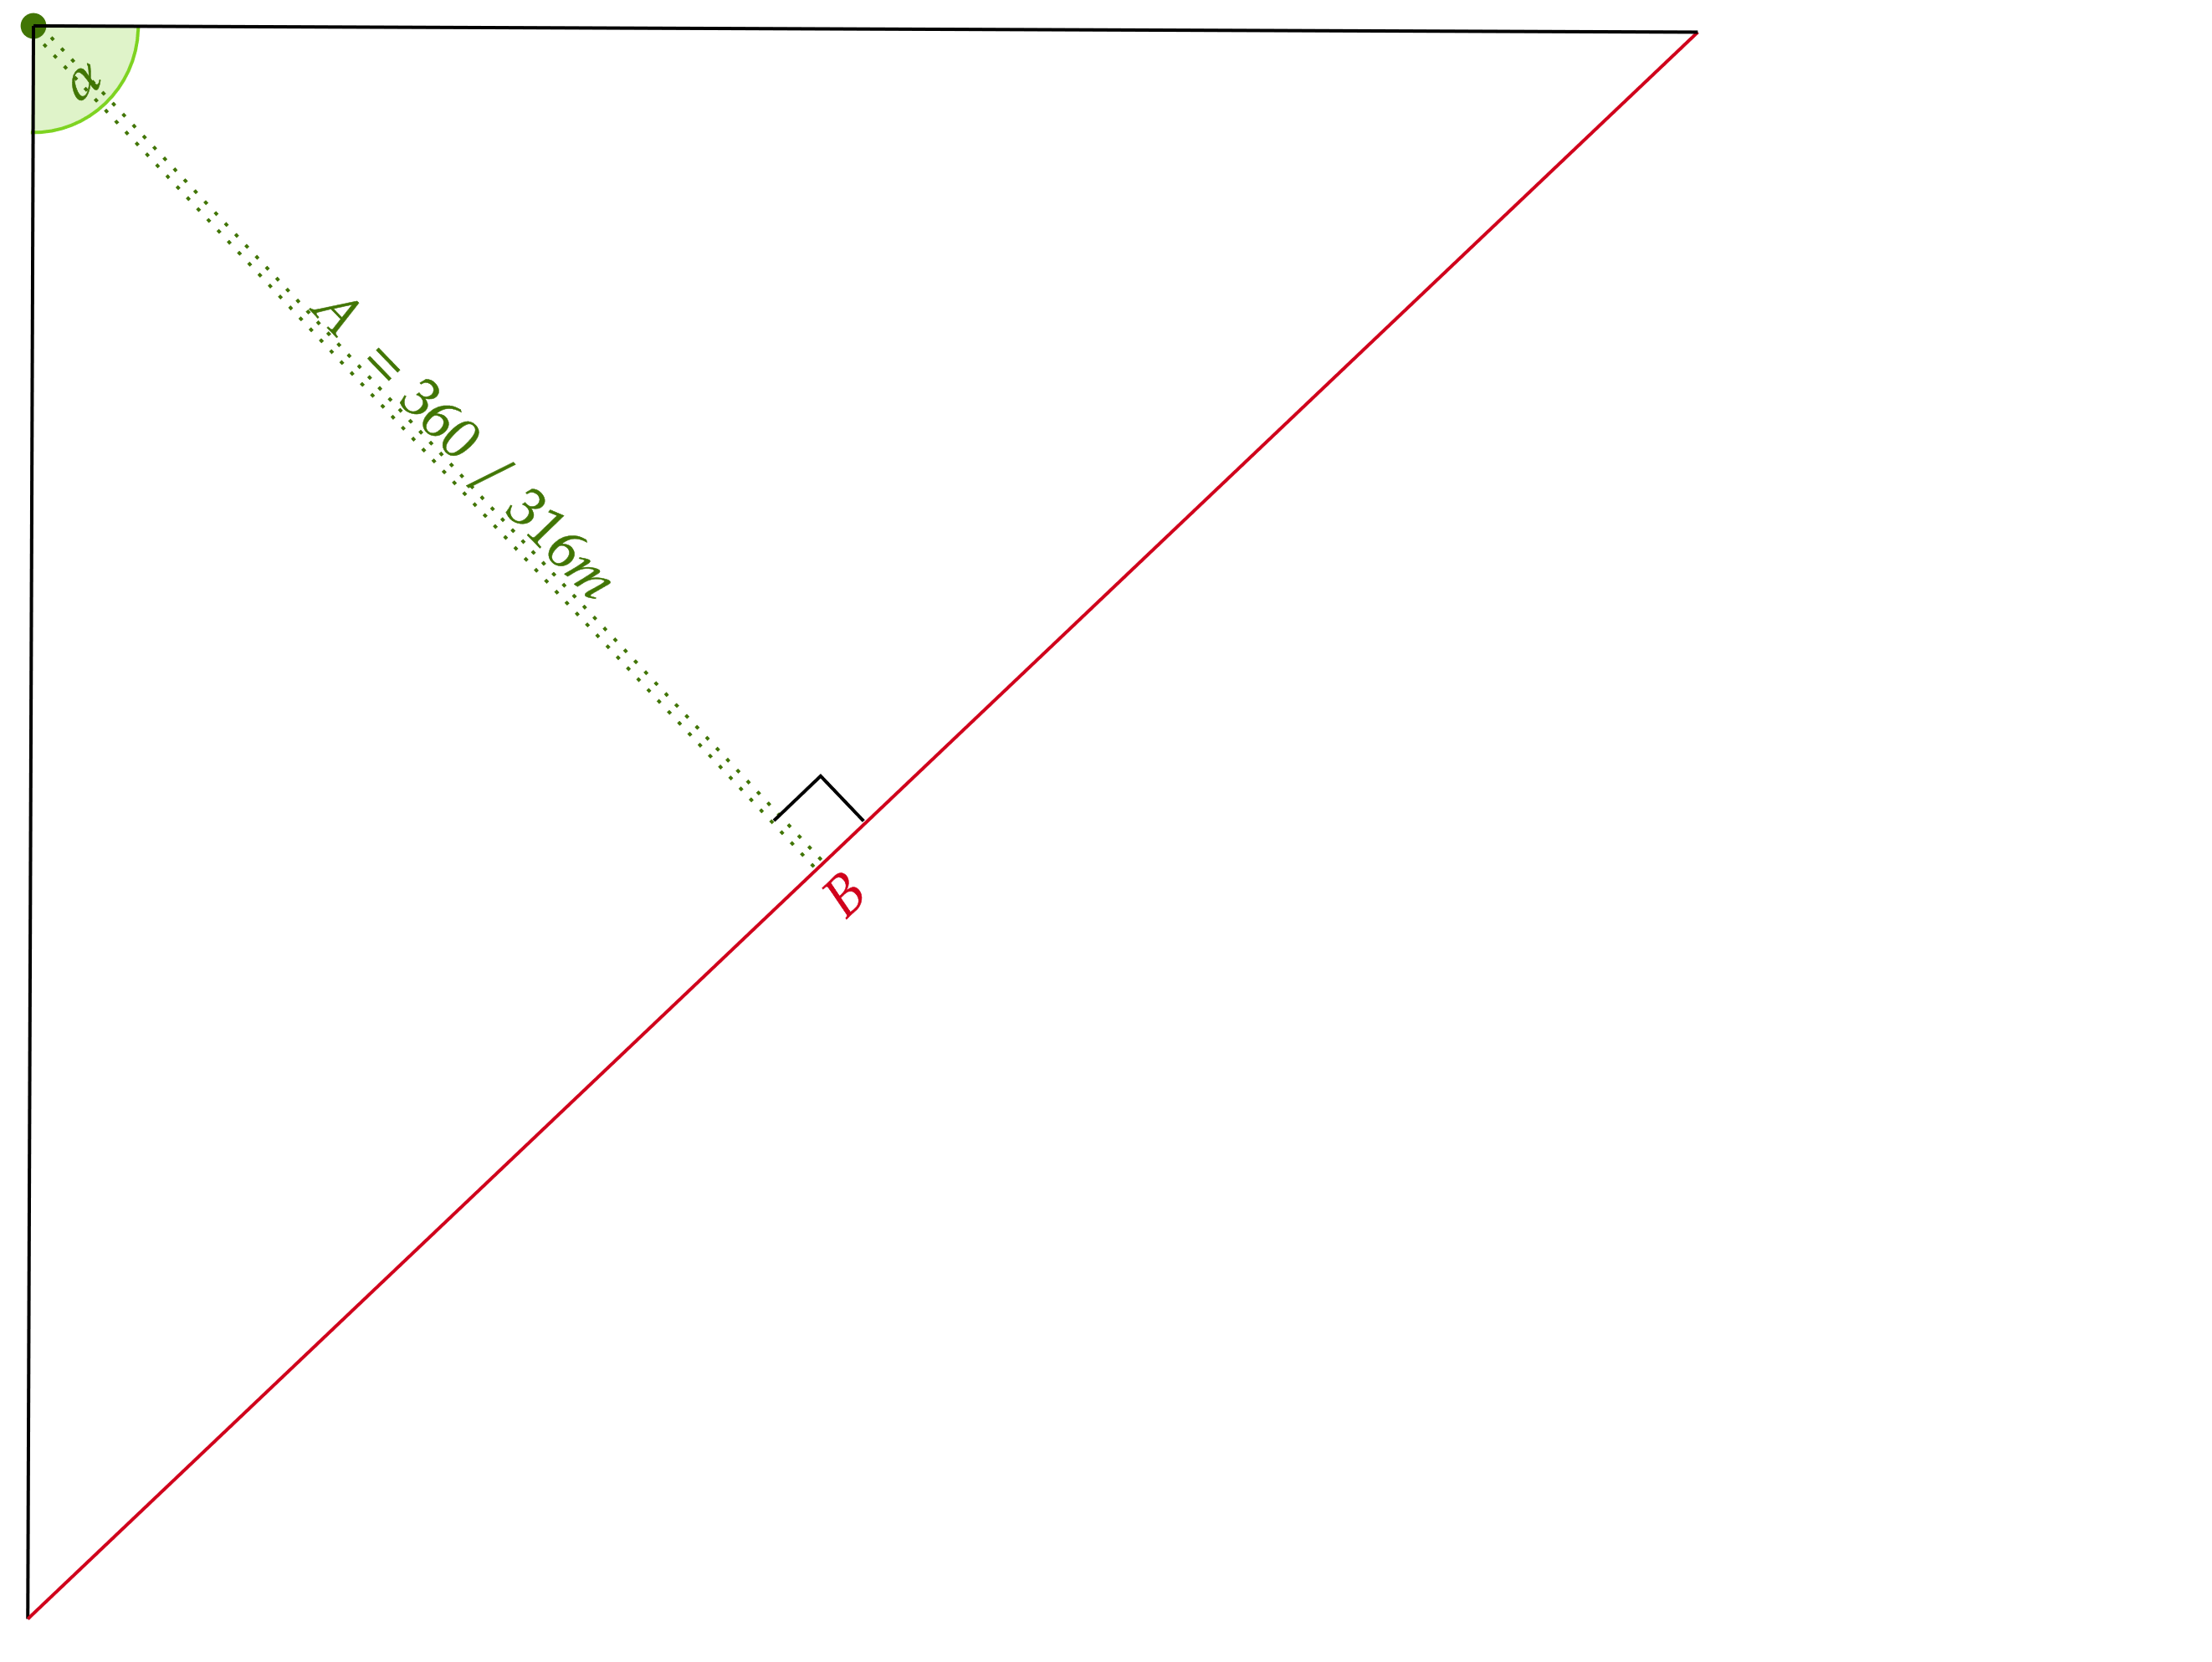
\includegraphics[width=0.9\textwidth]{figures/camera/horizontal.png}
%                 \captionof{figure}{Horizontales Sichtfeld}
%             \end{center}
%     \end{itemize}
% \end{mdframed}

% ****************************************************************************************************
